
\documentclass[a4paper,UTF8]{article}

 
%\usepackage{subfiles}

\usepackage{hyperref}

\usepackage{amsmath}
\usepackage{amsfonts}

\usepackage[a4paper,left=25mm,right=25mm,top=20mm,bottom=20mm]{geometry}

% \usepackage{ctex}

\usepackage{tikz}
\usepackage{pgfplots}
\usepackage{pgfplotstable}


\usepackage{fp}
\usepackage{graphicx}

\newtheorem{theorem}{定理}


\usepgfplotslibrary{colorbrewer}
\pgfplotsset{width=7cm,compat=1.13}


\begin{document}


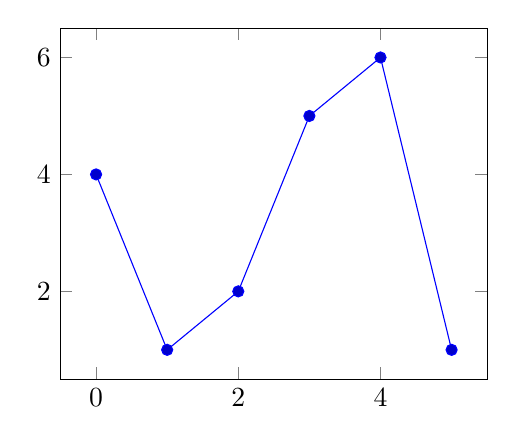
\begin{tikzpicture}                 % 绘图开始
\begin{axis}                        % 添加坐标
\addplot+[sharp plot]               % 调用绘图函数,并设置绘图的类型是折线图
coordinates                         % 声明是在迪卡尔坐标系中的数据
{                                   % 输入数据
 (0,4) (1,1) (2,2)
 (3,5) (4,6) (5,1)
};
\end{axis}                         % 结束坐标
\end{tikzpicture}                  % 绘图结束



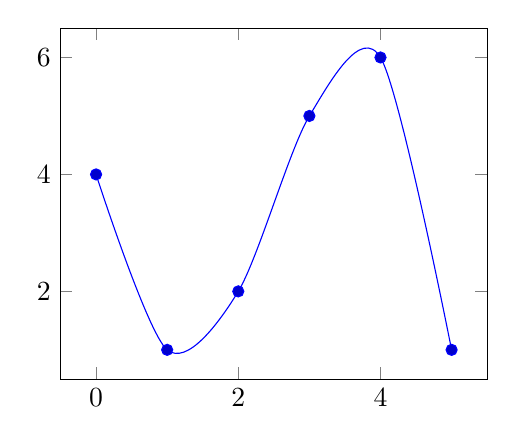
\begin{tikzpicture}
\begin{axis}
\addplot+[smooth]                    % 设置绘图的类型是光滑线图
coordinates
{
 (0,4) (1,1) (2,2)
 (3,5) (4,6) (5,1)
};
\end{axis}
\end{tikzpicture}



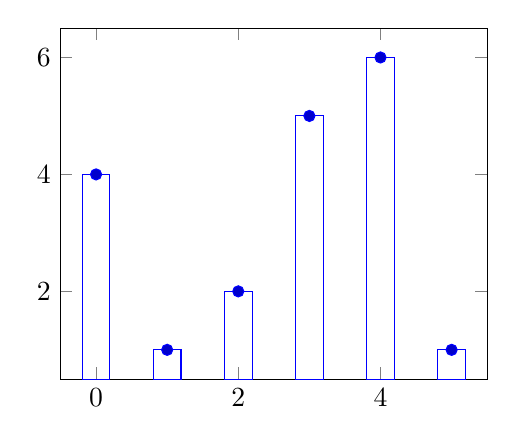
\begin{tikzpicture}
\begin{axis}
\addplot+[ybar]                      % 绘制关于y坐标的条形图
coordinates
{
 (0,4) (1,1) (2,2)
 (3,5) (4,6) (5,1)
};
\end{axis}
\end{tikzpicture}


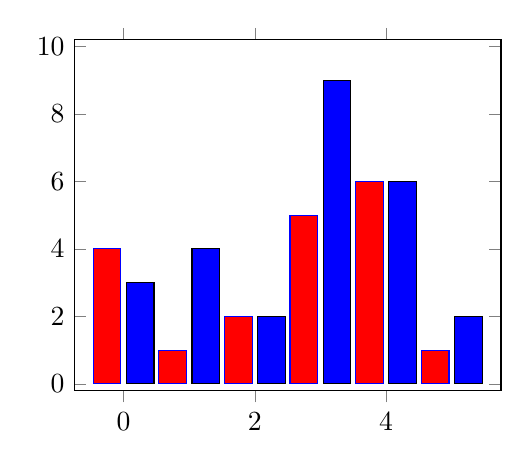
\begin{tikzpicture}
\begin{axis}[ybar,enlargelimits=0.15]  % 绘制关于y坐标的条形图,条形之间的最大间隔是0.15cm
\addplot[draw=blue,fill=red]           % 蓝色边界、红色填充
coordinates
{
 (0,4) (1,1) (2,2)
 (3,5) (4,6) (5,1)
};
\addplot[draw=black,fill=blue]         % 黑色边界、蓝色填充
coordinates
{
 (0,3) (1,4) (2,2)
 (3,9) (4,6) (5,2)
};
\end{axis}
\end{tikzpicture}

\begin{tikzpicture}
\begin{axis}[ybar interval]   % 绘制y条形图,并且分隔出区间
\addplot[hist={bins=3}]       % 绘制图像设置为直方图,组距为3
table[row sep=\\,y index=0]   % 设置表的行以"\\"分隔,y的从0开始
{
 data\\                       % 输入数据
 1\\ 2\\ 1\\ 5\\ 4\\ 10\\
 7\\ 10\\ 9\\ 8\\ 9\\ 9\\
};
\end{axis}
\end{tikzpicture}








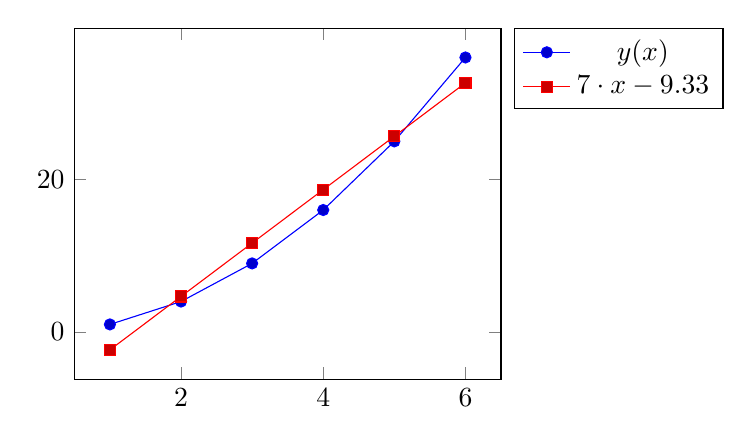
\begin{tikzpicture}
\begin{axis}[legend pos=outer north east] % 将图例放在图外,位于图的东北角
\addplot 
table                               % 绘制原始数据的折线图
{           		                % X,Y的原始数据
 X Y
 1 1
 2 4
 3 9
 4 16 
 5 25
 6 36
};
\addplot
table[y={create col/linear regression={y=Y}}] % 对输入的数据作线性回归
{   				
 X Y
 1 1
 2 4
 3 9
 4 16 
 5 25
 6 36
};
\addlegendentry{$y(x)$}          % 给第一个图像添加图例,即原始函数y(x)
\addlegendentry{                 % 给第二个图像添加图例,即线性回归结果a*x+b
$\pgfmathprintnumber{\pgfplotstableregressiona} \cdot x
\pgfmathprintnumber[print sign]{\pgfplotstableregressionb}$}
\end{axis}
\end{tikzpicture}




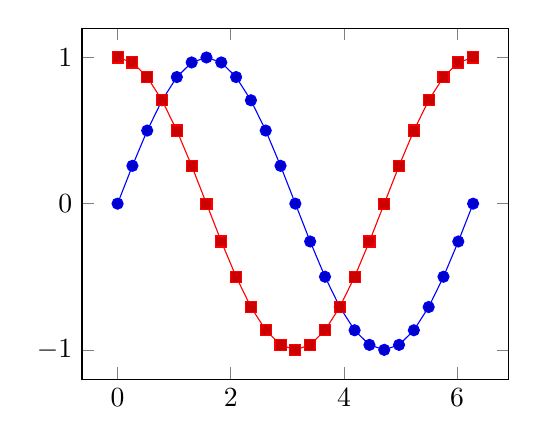
\begin{tikzpicture}
\begin{axis}
\addplot+[domain=0:2*pi]          % 设置函数的定义域
 {sin(deg(x))};                   % 输入显式函数
\addplot+[domain=0:2*pi]          % 设置函数的定义域
 {cos(deg(x))};                   % 输入显式函数
\end{axis}
\end{tikzpicture}





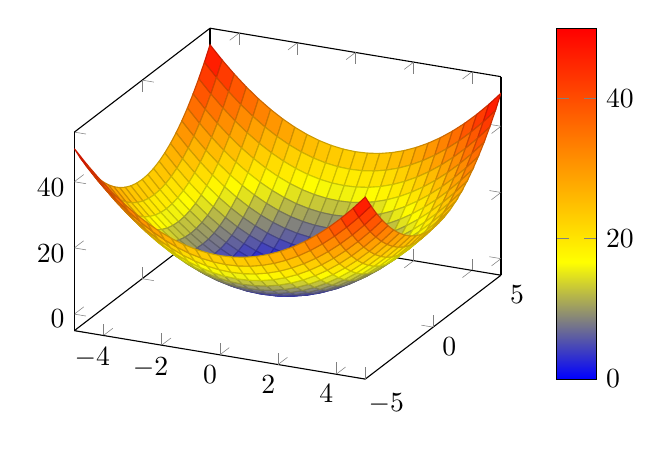
\begin{tikzpicture}
\begin{axis}[colorbar]         % 绘制坐标,并设置一个彩色指示条
\addplot3[surf]                % 绘制三维图
 {x^2+y^2};                    % 输入二元显式函数
\end{axis}
\end{tikzpicture}

\newpage

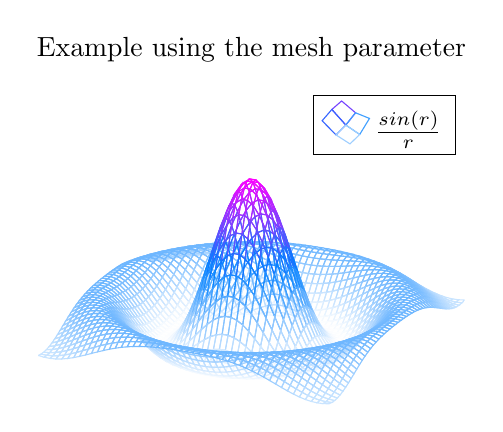
\begin{tikzpicture}
\begin{axis}[
    title=Example using the mesh parameter, %图像的标题
    hide axis,                              %隐藏坐标
    colormap/cool,                          %颜色风格
]
\addplot3[
    mesh,                                   %绘制的三维图像是网格
    samples=50,                             %定义域分割数量
    domain=-8:8,                            %定义域
]
{sin(deg(sqrt(x^2+y^2)))/sqrt(x^2+y^2)};    %二元显式函数
\addlegendentry{$\frac{sin(r)}{r}$}         %添加图例
\end{axis}
\end{tikzpicture}

\newpage

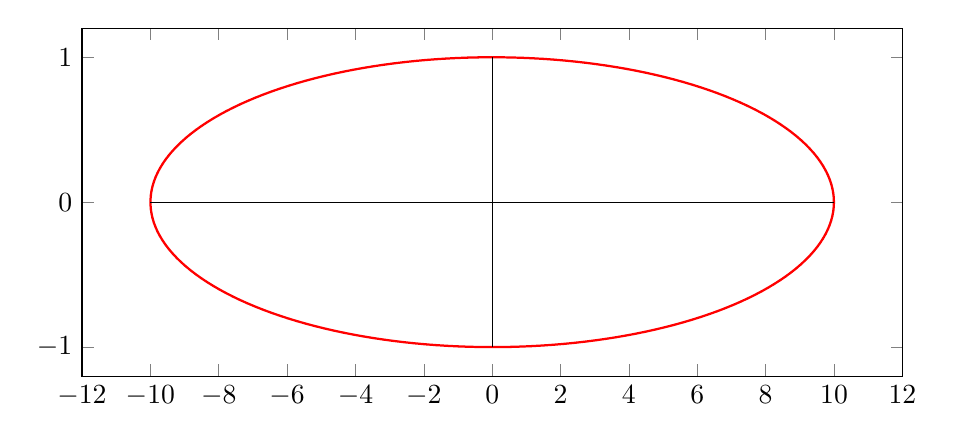
\begin{tikzpicture}
\begin{axis}[width=12cm,height=6cm,trig format plots=rad,variable=t]
\addplot[red,thick,domain=-2*pi:2*pi,samples=200]
({10*cos(t)},{sin(t)});
\draw (0,1) -- (0,-1) (-10,0) -- (10,0);
\end{axis}
\end{tikzpicture}

\end{document}

